\documentclass[alpha-refs]{wiley-article}

\usepackage[T1]{fontenc}
\usepackage[utf8]{inputenc}
\usepackage[english]{babel}
\usepackage{graphicx}
\graphicspath{{figures/}}
\usepackage[space]{grffile}
\usepackage{latexsym}
\usepackage{textcomp}
\usepackage{longtable}
\usepackage{tabulary}
\usepackage{booktabs,array,multirow}
\usepackage{amsfonts,amsmath,amssymb}
\usepackage{natbib}
\usepackage{url}
\usepackage{hyperref}
\hypersetup{colorlinks=false,pdfborder={0 0 0}}
\usepackage{etoolbox}
\usepackage{placeins}
\usepackage{siunitx}

\makeatletter
\@ifundefined{@combinedblfloats}{}{%
  \patchcmd\@combinedblfloats{\box\@outputbox}{\unvbox\@outputbox}{}{}%
}
\makeatother

\newif\iflatexml\latexmlfalse
\providecommand{\tightlist}{\setlength{\itemsep}{0pt}\setlength{\parskip}{0pt}}
\providecommand{\doi}[1]{\url{https://doi.org/#1}}
\AtBeginDocument{\DeclareGraphicsExtensions{.pdf,.PDF,.eps,.EPS,.png,.PNG,.tif,.TIF,.jpg,.JPG,.jpeg,.JPEG}}

\iflatexml
\else
\paperfield{Systems engineering; model-based systems engineering; nanosatellites; electrical power systems}
\abbrevs{EPS, electrical power system; MBSE, model-based systems engineering; PRISMA, Preferred Reporting Items for Systematic Reviews and Meta-Analyses; RQ, research question; SIL, software-in-the-loop; HIL, hardware-in-the-loop; V\&V, verification and validation}
\corraddress{Corresponding author details to be supplied before submission.}
\corremail{email-to-be-supplied@example.com}
\fundinginfo{Funding information to be supplied before submission.}
\fi

\papertype{Original Article}
\title{TBD}
\author[1]{Author Information To Be Supplied}
\affil[1]{Affiliation to be supplied}
\runningauthor{Author et al.}

\begin{document}

\maketitle
\selectlanguage{english}

\section{Methodology}

\subsection{Protocol and research questions}
This review used a predefined protocol to delimit the population, intervention, outcomes, eligibility criteria, and synthesis approach.  The protocol defines a nanosatellite-class population, an MBSE intervention, and outcomes concerned with general modeling, EPS-relevant value, and verification before physical development.  The review method is intentionally narrower than broad space-MBSE syntheses: Buruso et al. \cite{Buruso2026MBSESpace} are used as a methodological and positioning comparator, especially for transparent review procedure and concise enabler classification, but their review is not treated as evidence about the studies included here.

The protocol research questions were:
\begin{description}
\item[RQ1.] How can nanosatellite missions and EPS be modeled in a general manner with minimal knowledge about their behavior?
\item[RQ2.] What are the claimed outcomes related to reliability, reproducibility, and integrability derived from EPS modeling in nanosatellite missions?
\item[RQ3.] How have verification procedures been integrated into EPS models prior to physical development?
\end{description}

The population was interpreted as CubeSat and nanosatellite-class missions rather than larger spacecraft or smaller educational platforms such as CanSats.  For RQ1, the focal intervention was system-level or EPS-level MBSE.  For RQ2, outcomes had to be attributable to MBSE artifacts, MBSE activities, or model-enabled process changes rather than to the selected EPS technology alone.  For RQ3, the review looked for requirements, verification, validation, IVV, test, simulation, or analysis artifacts integrated in or around the model before hardware development.

\clearpage
\subsection{Information sources and search strategy}
Records were retrieved from Scopus and IEEE Xplore.  Scopus searches were run directly, while IEEE Xplore records were exported and screened using the same eligibility criteria.  Targeted exact-title Google Scholar searches were used only to verify or recover known titles identified through citation chasing; Google Scholar was not used as an open-ended third database.

Search strings combined nanosatellite/CubeSat population terms with MBSE terms such as ``model-based systems engineering'', MBSE, SysML, and selected alternative terminology including Capella, Arcadia, and cyber-physical systems where relevant.  The search strategy followed four concept clusters derived from the protocol: (i) general nanosatellite or CubeSat MBSE reference models, templates, behavior models, and mission/system architectures; (ii) EPS, power-subsystem, power-budget, and electrical-architecture modeling; (iii) verification, validation, IVV, test, requirements-in-the-loop, and traceability; and (iv) outcome and integration terms such as reliability, reproducibility, integrability, interoperability, and lifecycle continuity.  The final record set combined database search results, eligible IEEE Xplore records, and targeted citation-chasing recoveries.

Search and screening limits followed the protocol: publication years 2013--2026, English language, conference or journal papers, and either open access or availability through institutional library access.  Search details were recorded for query identifiers, query strings, result totals, recovery searches, and stopping rationale.  The stopping decision was based on saturation of the Scopus--IEEE evidence base and on the observation that later EPS/V\&V recall passes mainly confirmed sparsity rather than uncovering a large hidden literature.

\subsection{Selection process and eligibility criteria}
Records from the retained searches were merged and deduplicated before screening.  The final PRISMA-style flow was: 199 records identified, 118 duplicates removed, 81 unique records screened, 37 records excluded during screening, 44 reports sought for retrieval, 4 reports not retrieved or inaccessible, and 40 reports extracted.

Screening applied the protocol criteria as follows:
\begin{itemize}
\item include English conference or journal papers from 2013--2026;
\item include CubeSat, nanosatellite, or very close nanosatellite-class system-design studies, and exclude larger generic spacecraft, payload-only, ground-segment-only, software-only, hardware-calibration, education/tutorial, proceedings-volume, and non-space records unless a specific protocol-based rationale supported retention;
\item include studies using MBSE, SysML, model-based architecture, model-based requirements, model-based simulation/analysis, or closely related digital-engineering approaches at system level, mission level, EPS level, or an EPS-adjacent power/electrical-architecture level;
\item for RQ1, prioritize system-level or EPS-level models, reference models, templates, reusable workflows, behavior models, and architecture models over isolated subsystem models;
\item for RQ2, retain claimed outcomes only when the outcome could be linked to MBSE artifacts or model-enabled processes, not merely to EPS component choices;
\item for RQ3, require explicit verification, validation, IVV, test, requirements traceability, simulation, parametric checking, or pre-physical-development evaluation evidence in or around the model.
\end{itemize}

Screening distinguished core and supporting studies.  Core papers directly shaped the synthesis because they were central to CubeSat/nanosatellite MBSE, EPS/power modeling, traceability, reusable reference models, or V\&V.  Supporting papers were retained when they provided contextual evidence on toolchains, lifecycle continuity, requirements-in-the-loop, risk, project-management, or related nanosatellite MBSE practices without being as central to the protocol RQs.

\subsection{Data extraction and quality appraisal}
Extraction was performed on the 40 accessible reports, comprising 21 core and 19 supporting studies.  The four reports that remained inaccessible at retrieval were classified as unavailable and excluded from the evidence synthesis.

A standardized extraction form was used for every accessible study and was refactored into two linked layers.  First, a controlled codebook was derived from the protocol and used for synthesis-critical fields with explicit allowed values, including RQ relevance, lifecycle stage, EPS relevance, model maturity, modeling scope, MBSE approach classification, toolchain mechanisms, EPS/V\&V artifacts, outcome categories, evidence types, gap mapping, quality ratings, limitation flags, and extraction confidence.  Second, open extraction preserved researcher observations, unexpected mechanisms, tools, claims, caveats, and emergent themes that did not fit the controlled vocabulary.  Extracted fields covered bibliographic metadata; research-question relevance; mission/platform context; lifecycle stage; EPS relevance; model maturity; MBSE objective, scope, engineering artifacts, abstraction level, and reuse mechanism; implementation pathway and tailoring; toolchain, interoperability, and lifecycle-continuity mechanisms; EPS and verification-specific evidence; claimed outcomes, mechanisms, evidence types, metrics, baselines, and confidence ratings; governance, ROI, deliverables, and project-decision linkage; gap mapping; limitations; supporting quotations; lineage notes; and extraction confidence.

Each per-study extraction therefore contains both a compact controlled-code summary for aggregation and open `emergent codes' for qualitative synthesis.  Controlled codes were assigned only when the surrounding meaning supported the classification; keyword presence alone was not treated as evidence.  Values coded as ``other'' in controlled fields were retained as ``other'' and explained through emergent codes rather than silently expanding the codebook.  Limitation flags were used only for aggregation, while author-stated and extractor-identified limitation rationales were retained as text.

Quality appraisal used the protocol checklist rather than an exclusion threshold.  Each checklist item was scored as No = 0, Insufficiently = 0.5, or Yes = 1.  The checklist assessed venue credibility; whether limitations, threats, assumptions, or scope boundaries were discussed; clarity of nanosatellite/CubeSat context and lifecycle stage; clarity of MBSE method, language, toolchain, model artifacts, and system boundary; whether claimed outcomes were explicitly linked to MBSE artifacts or activities; whether evidence was provided for claims; whether requirements, verification, validation, design decisions, or lifecycle gates were traced to model artifacts when relevant; and whether model availability, reusable assets, data exchange, or implementation details were reported.  Quality scores were used to inform sensitivity, confidence, and discussion of evidence strength; they were not used to automatically remove studies after full-text extraction.

No independent inter-rater reliability assessment was performed.  Consequently, the review does not report agreement statistics.  Instead, extraction consistency was supported by the fixed protocol, a common extraction form, explicit rationales and direct quotes for coding decisions, extraction-confidence ratings, and cross-checking extracted data against source reports and eligibility decisions.

\subsection{Synthesis strategy}
The synthesis was structured by the three protocol RQs rather than by a general MBSE tool or method taxonomy.  Descriptive statistics were used to summarize study characteristics, study role (core or supporting), EPS relevance, approach classifications, quality-score distribution, research-question relevance, value-claim evidence, and V\&V linkage categories.  Narrative synthesis then interpreted these counts in relation to the protocol questions.

A concise enabler taxonomy was retained only as a secondary explanatory layer.  The Pure, Enhanced, Extended, and Integrated MBSE/digital-engineering categories, together with lifecycle activity anchors such as requirements management, model development, simulation/analysis, configuration management, and collaboration/communication, were used as sensitizing categories consistent with the broader space-MBSE review style of Buruso et al. \cite{Buruso2026MBSESpace}.  The main synthesis, however, focused on two issues specific to this review: the evidence behind claimed value and the linkage between MBSE artifacts and V\&V before physical development.

For RQ1, studies were compared by modeling focus: whole-nanosatellite models that include EPS or power as a subsystem, generic whole-nanosatellite models without explicit EPS, and EPS-only or EPS-first models.  Reuse mechanisms such as reference models, templates, profiles, libraries, open packages, and repeatable workflows were examined as evidence for generality and for modeling with limited prior behavioral knowledge.  For RQ2, each value claim was synthesized by controlled outcome category, specificity, MBSE mechanism, evidence type, metric or value indicator, baseline or comparator, and evidence-confidence rating.  Multi-label outcome-domain counts were derived from controlled outcome codes only, not from loose keyword searches over claim text; open observations were retained separately as emergent codes for qualitative interpretation.  This prevented asserted benefits such as reliability, reproducibility, integrability, schedule reduction, or communication improvement from being treated as measured effects unless the extraction recorded supporting evidence.  For RQ3, V\&V linkage was synthesized from controlled V\&V artifact, pre-physical verification, and integration/test-readiness codes, including requirements-to-model traceability, verification matrices, parametric and power-budget checks, executable simulation or scenario analysis, test cases and procedures, automated tests, external tool/data-flow coupling, and evidence of physical, software-in-the-loop, hardware-in-the-loop, or integration-test readiness.

\subsection{Review validity}
Several measures were used to strengthen review validity while preserving the limits of the available evidence base.  Construct validity was supported by deriving eligibility, extraction fields, and synthesis categories from the protocol RQs and by keeping the broad space-MBSE review \cite{Buruso2026MBSESpace} as a positioning reference rather than as evidence about the included studies.  Search validity was supported by using two major engineering bibliographic sources, exact query logging, deduplication, targeted recall searches for EPS/V\&V sparsity, IEEE parity checks, and citation-chasing recovery for specific missing titles.  The main search limitation is that the database scope was restricted to Scopus and IEEE Xplore, with Google Scholar used only for targeted exact-title verification, so grey literature and some publisher-specific records may be underrepresented.

Selection validity was supported by explicit inclusion/exclusion criteria and recorded screening decisions.  Residual uncertainty remains for records with limited abstracts, borderline eligibility decisions, and inaccessible reports.  Extraction validity was supported by full-text extraction for accessible studies, supporting quotations, quality appraisal, claim-evidence coding, and extraction-confidence ratings.  The absence of an independent inter-rater assessment is a limitation; no reliability statistic is claimed.

Synthesis validity was addressed by separating descriptive study patterns from evidence-backed findings.  Repeated publications from the same CubeSat reference-model lineage were treated with lineage notes so that publication count would not be mistaken for independent replication.  Claims about MBSE value were interpreted through evidence confidence and baseline availability, and EPS-specific conclusions were kept conservative because the evidence base contains many system-level or EPS-adjacent studies but few direct EPS-first studies.  External validity is therefore limited to nanosatellite/CubeSat-class MBSE under the search scope and should not be generalized to all space MBSE practice or to all spacecraft EPS development without further evidence.

\section{Results}
\label{sec:results}

\subsection{Search, screening, retrieval, and extraction flow}
\label{sec:results-flow}

The final synthesis included the 40 accessible studies that underwent standardized full-text extraction.  The review flow was: 199 records identified, 118 duplicates removed, 81 unique records screened, 37 records excluded during screening, 44 reports sought for retrieval, 4 reports not retrieved or inaccessible, and 40 reports extracted.  Unretrieved reports were excluded from the evidence synthesis.

\begin{figure}[htbp]
\centering
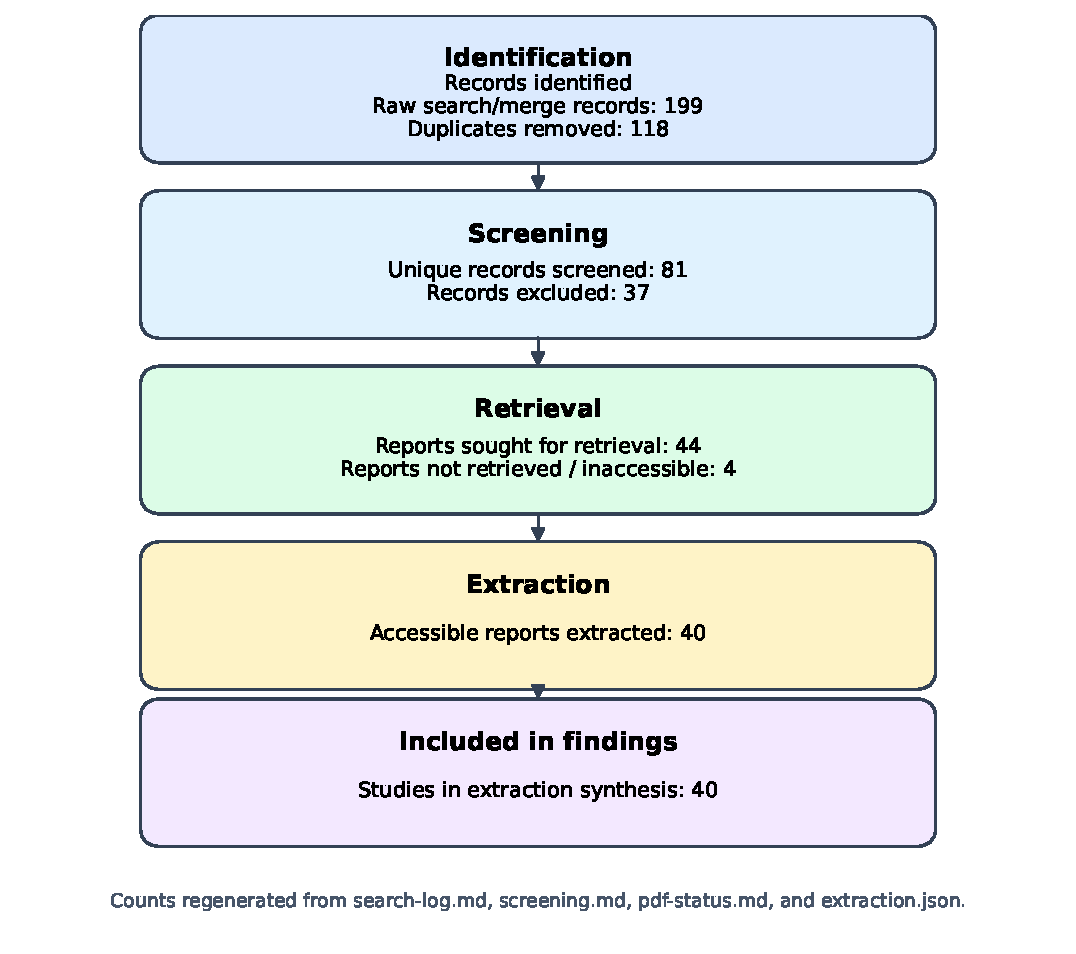
\includegraphics[width=0.78\linewidth]{prisma_flow}
\caption{Flow of record identification, screening, retrieval, and inclusion for the review synthesis.}
\label{fig:results-prisma-flow}
\end{figure}

The extracted set comprised 21 core studies and 19 supporting studies published from 2013 to 2025.  Counts below therefore refer to the 40 extracted studies unless identified as multi-label claim-domain or V\&V-linkage counts.

\subsection{Study characteristics and quality}
\label{sec:results-characteristics-quality}

The quality checklist scores ranged from 5.0 to 7.5 on the eight-item scale, with a mean of 6.21.  The score distribution was 5.0 ($n=3$), 5.5 ($n=6$), 6.0 ($n=13$), 6.5 ($n=9$), 7.0 ($n=7$), and 7.5 ($n=2$).  Extraction confidence was coded as high for 29 studies and medium for 11 studies.  RQ relevance was uneven: RQ1 was high for 24 studies and partial for 16; RQ2 was high for 3 and partial for 37; and RQ3 was high for 2, partial for 29, and not relevant for 9.  The mostly partial RQ2 pattern reflects that most papers stated MBSE value claims but did not directly measure EPS reliability, reproducibility, or integrability outcomes.

\begin{table}[htbp]
\centering
\caption{Study, quality, and claim-evidence summary.}
\label{tab:results-study-quality-summary}
\begin{tabular}{lr}
\toprule
Metric & n \\
\midrule
Extracted studies & 40 \\
Core studies & 21 \\
Supporting studies & 19 \\
Publication year range & 2013--2025 \\
Claim records & 270 \\
Unsupported claims & 52 \\
Weak claims & 139 \\
Moderate claims & 77 \\
Strong claims & 2 \\
High-confidence extractions & 29 \\
Medium-confidence extractions & 11 \\
\bottomrule
\end{tabular}
\end{table}

Structured limitation flags further contextualize quality.  The dominant limitations were incomplete lifecycle coverage ($n=40$), weak claim--evidence linkage ($n=40$), single-case or limited-scope evidence ($n=40$), no independent validation ($n=40$), prototype or future-work maturity ($n=40$), no physical-test or flight evidence ($n=39$), no baseline or comparator ($n=38$), no quantitative evaluation ($n=35$), unavailable model assets ($n=34$), no EPS-specific evidence ($n=33$), interoperability limitations ($n=29$), and no pre-physical verification model ($n=20$).  These flags were treated as evidence-strength constraints rather than as exclusion criteria, and open limitation text was retained separately from the aggregation flags.

\subsection{Modeling focus and EPS relevance}
\label{sec:results-modeling-focus-eps}

Modeling focus and EPS relevance were synthesized as a single mutually exclusive classification.  Thirty-four studies contained some EPS or power relevance: 19 reported concrete power-budget or electrical-architecture artifacts, 13 were EPS-adjacent, and 2 treated the EPS itself as the primary model scope.  The remaining 6 studies did not model EPS explicitly: 4 were system-level nanosatellite or CubeSat MBSE studies without power-specific artifacts, and 2 contributed nanosatellite MBSE or V\&V evidence outside the EPS domain.

\begin{figure}[htbp]
\centering
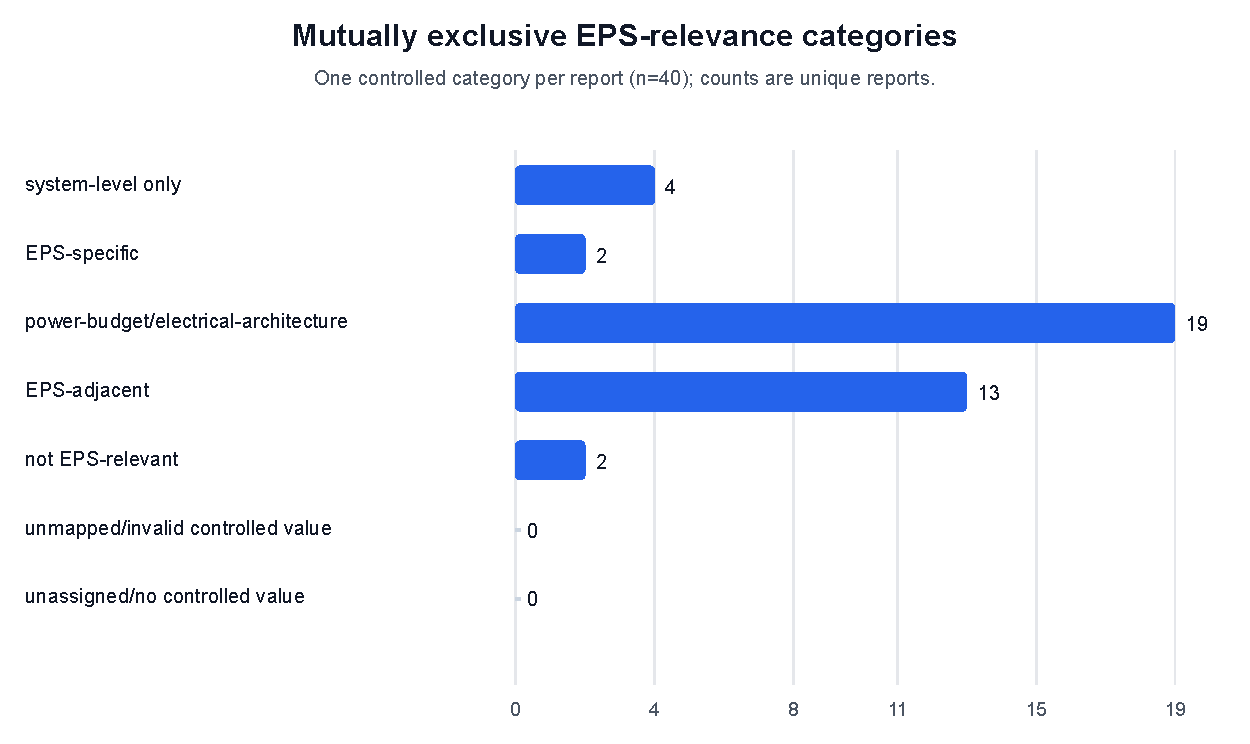
\includegraphics[width=0.78\linewidth]{eps_relevance_counts}
\caption{Mutually exclusive EPS relevance categories in the included studies.}
\label{fig:results-eps-relevance}
\end{figure}

\begin{table}[htbp]
\centering
\caption{Modeling focus and EPS relevance categories.}
\label{tab:results-eps-relevance-counts}
\begin{tabular}{lr}
\toprule
EPS relevance category & n \\
\midrule
Power-budget/electrical-architecture & 19 \\
EPS-adjacent & 13 \\
System-level only & 4 \\
EPS-specific & 2 \\
Not EPS-relevant & 2 \\
\bottomrule
\end{tabular}
\end{table}

The 19 power-budget/electrical-architecture studies should therefore be read as studies with concrete power-related evidence, not as 19 EPS-centered MBSE studies.  Most of this evidence was embedded in system-level models or preliminary design studies.  Examples include RAX/CubeSat energy and data simulations \cite{paper-0001,paper-0003,paper-0008}, SysML parametric mass and power-margin checks \cite{paper-0080}, Capella/Arcadia preliminary EPS allocation for 3ColStar \cite{paper-0078}, CNES concurrent electrical-architecture simulations \cite{paper-0053}, and PLM/Dymola requirements-in-the-loop power simulations \cite{paper-0059}.  The two EPS-specific studies were the open-source Papyrus/SysML power-subsystem model with Java-based parameter and requirement-traceability extraction \cite{paper-0026} and the requirements-in-the-loop PLM/Dymola CubeSat case in which EPS behavior and state-of-charge simulation were central \cite{paper-0059}.  Not-EPS-relevant studies still contributed general nanosatellite MBSE or V\&V evidence, such as the EIRSAT-1 communications-subsystem verification demonstrator \cite{paper-0063}.

This synthesis is intentionally stricter than simply counting any paper that mentioned power or included a generic EPS block.  EPS appeared frequently as a system concern, but direct EPS-first MBSE evidence remained sparse even after the refactored extraction separated EPS-specific, EPS-adjacent, and power-budget evidence.

\subsection{MBSE approaches, languages, and toolchains}
\label{sec:results-approaches-tools}

Approach classification was dominated by extended and enhanced MBSE rather than fully integrated digital-engineering environments.  Seventeen studies were coded as Extended MBSE, 11 as Enhanced MBSE, 6 as Integrated MBSE/digital engineering, and 6 as Pure MBSE.  This distribution situates the evidence base but does not by itself establish value or V\&V effectiveness.

\begin{table}[htbp]
\centering
\caption{MBSE approach-classification counts.}
\label{tab:results-approach-counts}
\begin{tabular}{lr}
\toprule
Approach classification & n \\
\midrule
Extended MBSE & 17 \\
Enhanced MBSE & 11 \\
Integrated MBSE/digital engineering & 6 \\
Pure MBSE & 6 \\
\bottomrule
\end{tabular}
\end{table}

Tool and language classification showed a SysML-centered set of studies: SysML appeared in 28 studies, custom tools in 17, Cameo/MagicDraw/CATIA Magic in 14, MATLAB/Simulink and STK in 10 each, open-source packages in 9, ModelCenter and PLM/ALM tools in 6 each, Python in 5, Capella/Arcadia in 4, requirements tools in 4, and OpenMBEE in 3.  The high count for ``other'' tools in the controlled summary reflects named toolchains that were preserved as emergent codes rather than forced into loose categories.  Results-relevant toolchains included Papyrus/Eclipse for the EPS-specific open-source case \cite{paper-0026}, Gaphor/UML stereotypes for open-source preliminary-design formalization \cite{paper-0029}, docs-as-code/M30ML for SeaLion documentation and traceability \cite{paper-0037}, Dymola/Modelica in 3DExperience \cite{paper-0059}, and IDM-CIC/Simu-CIC/Opalis for electrical-architecture concurrent engineering \cite{paper-0053}.

Toolchain use was usually reported as a means to connect requirements, architecture, analysis, and verification artifacts.  The strongest toolchain evidence came from executable or data-flow demonstrations, such as MagicDraw/Cameo--ModelCenter--STK--MATLAB integrations for RAX-style CubeSat analysis \cite{paper-0001,paper-0003}, Capella/ForPlan or Capella/open-source simulation coupling \cite{paper-0033,paper-0043}, and SysML/PLM/Dymola requirements-in-the-loop simulation \cite{paper-0059}.  Pure reference-model studies reported reusable structures and V\&V packages, but generally provided less executed analysis evidence \cite{paper-0015,paper-0077}.

\subsection{Claimed outcomes and value-evidence strength}
\label{sec:results-claims-evidence}

We extracted 270 claim records.  Evidence confidence for those claims was classified as Unsupported ($n=52$), Weak ($n=139$), Moderate ($n=77$), and Strong ($n=2$).  The two strong claims both came from a single concurrent-model-based CubeSat mission-design study that reported a quantitative comparison with a traditional feasibility-study process \cite{paper-0061}.  Outcome domains are multi-label and are now derived from controlled outcome codes only; the 270 claims produced 727 claim-domain memberships.

\begin{figure}[htbp]
\centering
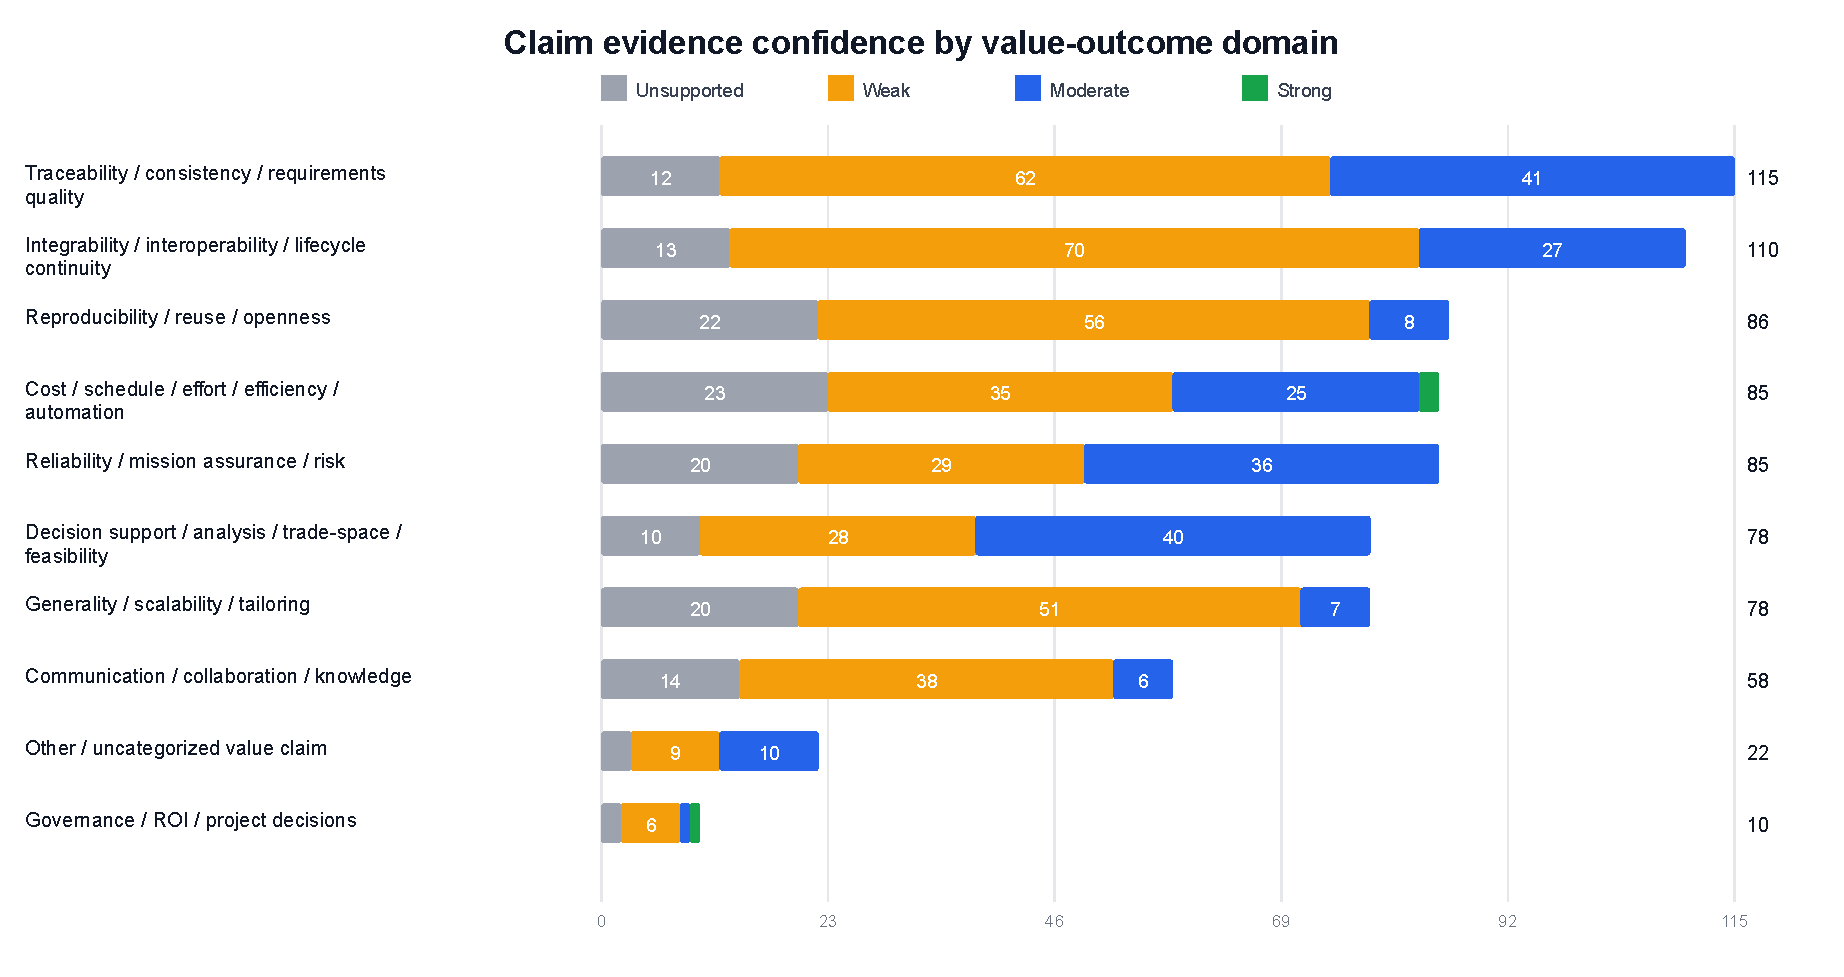
\includegraphics[width=0.92\linewidth]{claim_evidence_by_outcome}
\caption{Claim evidence by value-outcome domain.  Domains are multi-label, so counts exceed the number of unique claim records.}
\label{fig:results-claim-evidence}
\end{figure}

\begin{table*}[htbp]
\centering
\scriptsize
\caption{Claim evidence by value-outcome domain.  Domains are multi-label.}
\label{tab:results-claim-evidence-by-domain}
\begin{tabular}{p{0.47\linewidth}rrrrrr}
\toprule
Outcome domain & Total & Unsup. & Weak & Mod. & Strong & Studies \\
\midrule
Traceability / consistency / requirements quality & 115 & 12 & 62 & 41 & 0 & 37 \\
Integrability / interoperability / lifecycle continuity & 110 & 13 & 70 & 27 & 0 & 35 \\
Reproducibility / reuse / openness & 86 & 22 & 56 & 8 & 0 & 35 \\
Cost / schedule / effort / efficiency / automation & 85 & 23 & 35 & 25 & 2 & 33 \\
Reliability / mission assurance / risk & 85 & 20 & 29 & 36 & 0 & 33 \\
Decision support / analysis / trade-space / feasibility & 78 & 10 & 28 & 40 & 0 & 33 \\
Generality / scalability / tailoring & 78 & 20 & 51 & 7 & 0 & 34 \\
Communication / collaboration / knowledge & 58 & 14 & 38 & 6 & 0 & 34 \\
Other / uncategorized value claim & 22 & 3 & 9 & 10 & 0 & 9 \\
Governance / ROI / project decisions & 10 & 2 & 6 & 1 & 1 & 6 \\
\bottomrule
\end{tabular}
\end{table*}

The most frequent domains were traceability/consistency/requirements quality (115 memberships across 37 studies), integrability/interoperability/lifecycle continuity (110 across 35), reproducibility/reuse/openness (86 across 35), and cost/schedule/effort/automation and reliability/mission-assurance/risk (85 each across 33 studies).  EPS-specific or power-relevant claims were concentrated in integrability/interoperability (62 memberships), traceability/requirements quality (61), decision support (58), cost/schedule/effort/automation (53), reproducibility/reuse (47), and reliability/mission assurance/risk (46).  The explicit ``other'' category reflects the open-coding policy: observations that did not fit controlled outcome labels were preserved rather than reclassified through keywords.

Moderate evidence typically came from executed simulations, model-derived calculations, traceability artifacts, or case-study outputs.  Examples include the RAX model's energy/data interaction and solar-panel/battery sizing analyses \cite{paper-0001,paper-0003}, Papyrus/Java power-subsystem parameter-impact and requirement-fulfillment tables \cite{paper-0026}, power and SoC simulation against requirements in a PLM/Dymola workflow \cite{paper-0059}, worst-case battery survival simulation with a reported minimum state of charge in an electrical-architecture process \cite{paper-0053}, and positive mass/power margins from SysML parametrics \cite{paper-0080}.  Project-value metrics were rarer and case-specific, such as a one-month versus three-month feasibility-study comparison and lower estimated mission cost in one concurrent-design case \cite{paper-0061}, or the reported four-month preliminary-design cycle using Arcadia and weekly sprints \cite{paper-0078}.

Unsupported and weak claims were common where papers asserted reduced cost, reduced schedule, improved reliability, improved learning, or greater reuse without a baseline, metric, reuse trial, stakeholder evaluation, integration test, or flight/operational evidence.  For example, the EPS-specific Papyrus study provided moderate evidence for traceability and requirement-constraint checking, but its cost/time savings remained a future quantitative-benefit study rather than an observed outcome \cite{paper-0026}.  Reliability/mission-assurance/risk claims were more visible after controlled recoding than in the previous synthesis: 85 memberships were coded, with 36 moderate and none strong.  The two strong claims were not EPS-specific reliability claims; both concerned cost/schedule effects in a single concurrent-design feasibility comparison \cite{paper-0061}.

\subsection{Verification and validation linkage}
\label{sec:results-vv-linkage}

For V\&V, each study could receive multiple linkage categories based on controlled EPS/V\&V artifact, pre-physical verification, and integration/test-readiness codes.  EPS/power-specific pre-physical verification appeared in 25 studies; parametric, budget, or constraint checks in 23; executable simulation or scenario analysis before build in 22; test cases, procedures, or V\&V activity packages in 21; requirements-to-model traceability or verification matrices in 19; and external tool or data-flow coupling for V\&V in 11.  Twelve studies had no explicit EPS-focused pre-physical V\&V, 10 linked the model to physical, SIL/HIL, or integration-test readiness, and 3 had only generic or planned V\&V linkage.

\begin{figure}[htbp]
\centering
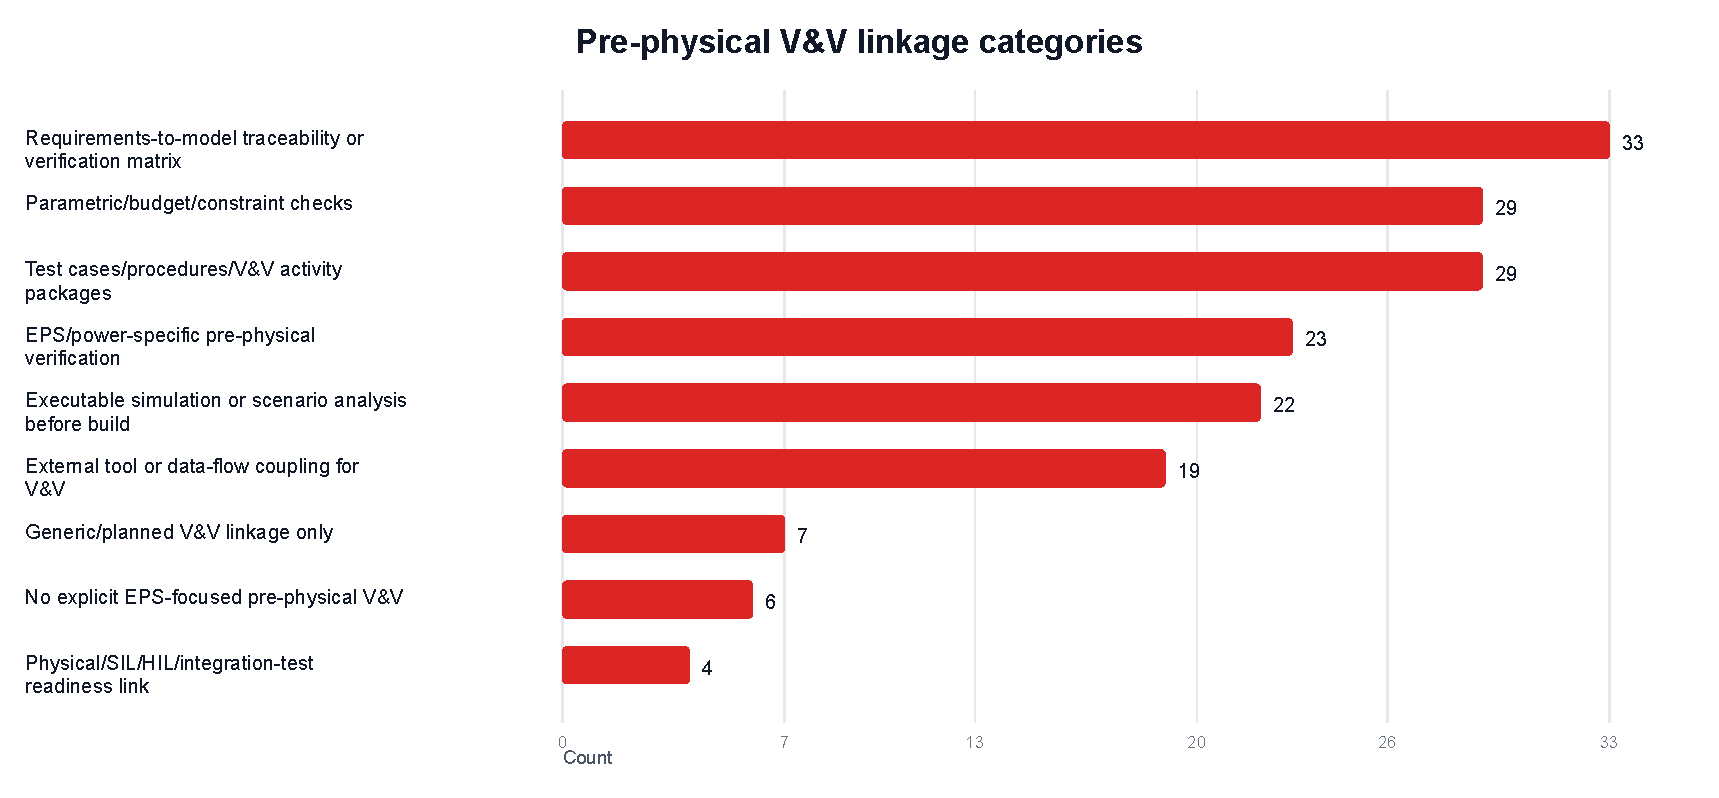
\includegraphics[width=0.92\linewidth]{vv_linkage_counts}
\caption{Pre-physical V\&V linkage categories.  Categories are multi-label by study.}
\label{fig:results-vv-linkage}
\end{figure}

\begin{table*}[htbp]
\centering
\scriptsize
\caption{Pre-physical V\&V linkage counts.  Categories are multi-label by study.}
\label{tab:results-vv-linkage-counts}
\begin{tabular}{p{0.68\linewidth}r}
\toprule
V\&V linkage category & n \\
\midrule
EPS/power-specific pre-physical verification & 25 \\
Parametric/budget/constraint checks & 23 \\
Executable simulation or scenario analysis before build & 22 \\
Test cases/procedures/V\&V activity packages & 21 \\
Requirements-to-model traceability or verification matrix & 19 \\
No explicit EPS-focused pre-physical V\&V & 12 \\
External tool or data-flow coupling for V\&V & 11 \\
Physical/SIL/HIL/integration-test readiness link & 10 \\
Generic/planned V\&V linkage only & 3 \\
\bottomrule
\end{tabular}
\end{table*}

Together, these categories show that V\&V was usually represented through EPS/power analysis, parametric checks, simulation, and planned or modeled test artifacts.  Explicit links from the model to test execution or integration evidence were still less common than pre-physical analysis, but the controlled recoding separated actual readiness links from generic V\&V language.

Requirements traceability was usually represented through SysML satisfy/verify relations, verification matrices, or tool-generated traceability views.  In the EPS-specific case, requirement constraints and power-budget equations were extracted from Papyrus and evaluated by Java, producing respected/not-respected flags \cite{paper-0026}.  In academic nanosatellite project modeling, requirements were linked to ``Verified By'' test cases and behavior diagrams such as Bus System Activation and LEOP flow \cite{paper-0023}.  In the 3ColStar preliminary design, EPS continuous-power requirements were traced to physical components such as solar panels and batteries \cite{paper-0078}.  In the NSS-1 SysML case, verify relationships connected mass and power requirements to constraint blocks, and positive margins were used as verification evidence \cite{paper-0080}.

Parametric and executable V\&V evidence was strongest when requirement checks were tied to simulation or budget outputs.  RAX/CubeSat studies executed mission scenarios and trade studies involving energy collection, battery capacity, solar-panel sizing, data storage, and downlink \cite{paper-0001,paper-0003,paper-0008}.  Later studies linked pre-physical V\&V to open-source model-to-analysis pipelines \cite{paper-0027,paper-0029,paper-0043}, PLM/Dymola requirements-in-the-loop simulation \cite{paper-0059}, and electrical-architecture energy-balance simulations before hardware development \cite{paper-0053}.  Test-case or automated-test evidence was more limited and often not EPS-specific, as in the requirements modeling/mapping matrix for CubeSat tests \cite{paper-0034} and the EIRSAT-1 communications verification model coupled to Python and ground-station hardware \cite{paper-0063}.  The physical/SIL/HIL/integration-test readiness category ($n=10$) was broader than completed hardware testing: most linkage still stopped at readiness, planned integration, or partial software/hardware interfaces rather than closed-loop EPS acceptance evidence.

\subsection{Gap mapping}
\label{sec:results-gap-mapping}

Each study was mapped to five gap categories adapted from the broader space-MBSE gap frame: practical implementation pathway; toolchain fragmentation/interoperability; lightweight/resource-constrained tailoring; governance/project deliverables/ROI/value; and NewSpace/agile/distributed/rapid iteration.  Classifications were coded as addressed with evidence, addressed conceptually, mentioned only, or not addressed.

\begin{figure}[htbp]
\centering
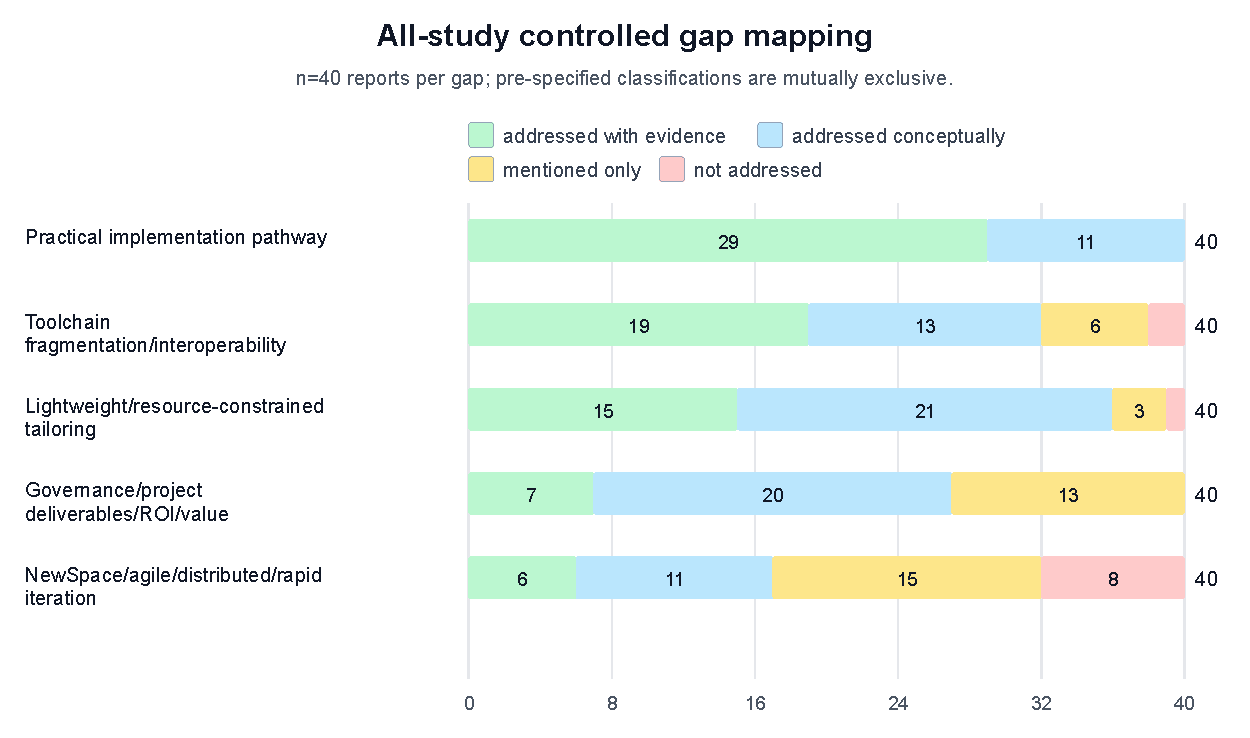
\includegraphics[width=0.92\linewidth]{gap_mapping_counts}
\caption{Gap-mapping counts for the extracted studies.}
\label{fig:results-gap-mapping}
\end{figure}

\begin{table*}[htbp]
\centering
\scriptsize
\caption{Gap mapping counts.}
\label{tab:results-gap-mapping-counts}
\begin{tabular}{p{0.46\linewidth}rrrr}
\toprule
Gap & Evidence & Conceptual & Mentioned & Not addressed \\
\midrule
Practical implementation pathway & 29 & 11 & 0 & 0 \\
Toolchain fragmentation/interoperability & 19 & 13 & 6 & 2 \\
Lightweight/resource-constrained tailoring & 15 & 21 & 3 & 1 \\
Governance/project deliverables/ROI/value & 7 & 20 & 13 & 0 \\
NewSpace/agile/distributed/rapid iteration & 6 & 11 & 15 & 8 \\
\bottomrule
\end{tabular}
\end{table*}

Implementation pathways were the most consistently addressed gap: all 40 studies addressed the pathway at least conceptually, with 29 evidence-backed and 11 conceptual classifications.  Evidence-backed examples included concrete modeling/data-flow steps for EPS traceability \cite{paper-0026}, concurrent electrical-architecture simulation workflow \cite{paper-0053}, and Capella/Arcadia plus agile preliminary-design execution \cite{paper-0078}.  Toolchain fragmentation/interoperability was also frequently addressed, with 19 evidence-backed cases, 13 conceptual cases, 6 mentioned-only cases, and 2 not-addressed cases.  Evidence-backed toolchain examples included executable RAX integrations \cite{paper-0001,paper-0003}, Papyrus-to-Java EPS analysis \cite{paper-0026}, open-source model-to-simulation coupling \cite{paper-0043}, and model-to-test/tool integration in EIRSAT-1 \cite{paper-0063}.

Lightweight/resource-constrained tailoring was addressed with evidence in 15 studies, addressed conceptually in 21, mentioned only in 3, and not addressed in 1.  Evidence-backed tailoring appeared in studies with rapid analytical design-space exploration \cite{paper-0012}, academic project-management and design tailoring \cite{paper-0023}, open/concurrent preliminary-design tooling \cite{paper-0027}, docs-as-code for a university CubeSat \cite{paper-0037}, causal MBSE user evaluation \cite{paper-0046}, low-cost tradespace modeling \cite{paper-0054}, and agile distributed preliminary design \cite{paper-0078}.

Governance, project deliverables, ROI, and value linkage remained weaker than implementation-pathway and toolchain evidence, but the controlled recoding identified 7 evidence-backed studies, 20 conceptual studies, and 13 mentioned-only studies.  Evidence-backed examples included the 3ColStar study, which reported Capella/Arcadia governance, weekly sprints, requirement/design traceability, and a four-month preliminary design cycle \cite{paper-0078}, as well as studies linking models to project deliverables, cost/schedule comparisons, or requirements-in-loop decision artifacts \cite{paper-0023,paper-0059,paper-0061}.  NewSpace/agile/distributed/rapid-iteration evidence was also limited, with 6 evidence-backed studies, 11 conceptual, 15 mentioned-only, and 8 not addressed.

\section{Discussion}
\label{sec:discussion}

\subsection{Relationship to the broader space-MBSE review}
\label{sec:discussion-buruso-relationship}

Buruso et al. provide the appropriate background for this review because their comprehensive space-MBSE synthesis already covers the broad distribution of MBSE methods, modeling languages, tools, lifecycle phases, and enabler classes across space applications \cite{Buruso2026MBSESpace}.  The present review therefore does not treat the recurrence of SysML, Cameo/MagicDraw, Capella/Arcadia, PLM tools, simulation environments, or integrated digital-engineering toolchains as a novel finding by itself.  Instead, those enablers are interpreted only where they affect nanosatellite and EPS-relevant value evidence, implementation burden, or model-linked V\&V.

The strongest connection to Buruso et al. is their discussion of value-driven implementation and their Table~5 research gaps.  They identify persistent gaps in practical implementation pathways, fragmented toolchains and lifecycle interoperability, resource-mismatched frameworks for small missions, weak linkage between MBSE artifacts, governance and ROI, and misalignment with NewSpace-style development needs \cite{Buruso2026MBSESpace}.  Our results support those gaps in a narrower population and make their nanosatellite consequences more explicit.  In the included studies, practical implementation pathways and toolchain interoperability are frequently addressed, with evidence-backed classifications in 29 and 19 studies respectively, but governance/ROI/value and NewSpace/agile/distributed development are less frequently addressed with evidence (7 and 6 studies respectively; Table~\ref{tab:results-gap-mapping-counts}).  Thus, the nanosatellite literature is not simply missing MBSE awareness; it is missing durable evidence that the models change project outcomes, review decisions, or downstream verification practice.

This narrower focus also exposes an EPS-specific asymmetry that is hidden in broad space-MBSE taxonomies.  Many studies include EPS or power concerns inside whole-CubeSat models, but only two included studies are EPS-specific or EPS-first \cite{paper-0026,paper-0059}.  Most examples of power modeling are embedded in system-level trade studies, reference-model work, or preliminary design workflows such as RAX energy/data simulation \cite{paper-0001,paper-0003}, SysML power-budget margins \cite{paper-0080}, Capella/Arcadia preliminary EPS allocation \cite{paper-0078}, PLM/Dymola battery simulation \cite{paper-0059}, and electrical-architecture concurrent engineering \cite{paper-0053}.  This extends Buruso et al.'s Table~5 concern about implementation pathways: for nanosatellites, the missing pathway is not only ``how to adopt MBSE,'' but how to maintain an EPS/system thread from mission objectives to power requirements, architectural allocation, analysis, verification procedure, and test evidence without imposing enterprise-scale overhead.

\subsection{Value-driven MBSE remains under-evidenced for nanosatellites}
\label{sec:discussion-value-evidence}

The review supports Buruso et al.'s claim that MBSE value must be tied to explicit objectives, model usage, governance, and evaluation criteria \cite{Buruso2026MBSESpace}.  The nanosatellite literature reviewed here contains many value claims, but the evidence is generally modest.  RQ2 was coded as high for only 3 studies and partial for 37, and among 270 extracted value-claim records only 2 were classified as strong evidence; 77 were moderate, 139 weak, and 52 unsupported (Table~\ref{tab:results-study-quality-summary}).  The most common domains were traceability, interoperability/lifecycle continuity, reproducibility/reuse, reliability/mission assurance, and cost/schedule/automation or decision-support mechanisms, but the strong evidence was confined to cost/schedule claims in one concurrent-design comparison rather than EPS reliability or verification closure (Table~\ref{tab:results-claim-evidence-by-domain}).

Moderate evidence usually came from executable demonstrations or traceable artifacts rather than from measured project outcomes.  For example, the RAX studies show how an integrated SysML--ModelCenter--STK--MATLAB workflow can simulate energy and data interactions, support solar-panel and battery-capacity trades, and check mission requirements \cite{paper-0001,paper-0003}.  The open-source Papyrus power-subsystem study demonstrates parameter-impact traceability and requirement-constraint flags from model data \cite{paper-0026}.  PLM/Dymola requirements-in-the-loop simulation reports battery state-of-charge behavior against an SoC requirement \cite{paper-0059}, and the electrical-architecture workflow reports a worst-case battery state-of-charge margin for survival/no-illumination conditions \cite{paper-0053}.  These are useful forms of engineering evidence, but they are mostly prototype, single-case, or pre-physical demonstrations.

Evidence becomes thinner when claims move from technical feasibility to project value.  Reported schedule or cost benefits exist, such as a one-month versus three-month feasibility-study comparison and lower estimated mission cost in a concurrent-design case \cite{paper-0061}, or a four-month preliminary-design cycle with Arcadia and weekly sprints for 3ColStar \cite{paper-0078}.  However, such claims are case-specific and rarely supported by controlled baselines, repeated use, independent stakeholder assessment, or lifecycle follow-through.  Similarly, reference models and templates promise reuse and consistency \cite{paper-0011,paper-0015,paper-0077}, while docs-as-code and open-source workflows improve accessibility and reproducibility \cite{paper-0037,paper-0029}, but the included studies seldom demonstrate reuse across independent missions or quantify the effort required to maintain the model.

The implication is that nanosatellite MBSE remains more artifact-driven than value-driven.  Studies frequently show that a model can contain requirements, architectures, budgets, interfaces, simulations, or generated documents.  Fewer studies define the mission/project objective that justifies the modeling effort, the metric used to evaluate success, the baseline practice being improved, or the review gate at which the model changes a decision.  This is especially important for EPS: power budgets, SoC traces, and margin checks are often convincing local analyses, but they are not always connected to explicit mission assurance objectives such as survival probability, operational availability, fault tolerance, or verification closure.  In this respect, our synthesis directly supports Buruso et al.'s Table~5 gap on weak integration between MBSE artifacts, governance, ROI, and value realization, and shows that the gap persists even in a domain where resource constraints should make value justification central \cite{Buruso2026MBSESpace}.

\subsection{V\&V linkage is present but rarely continuous}
\label{sec:discussion-vv-continuity}

The included studies do not show an absence of V\&V linkage; rather, they show many partial linkages that rarely form a continuous model-to-test thread.  EPS/power-specific pre-physical verification appeared in 25 studies, parametric/budget/constraint checks in 23, executable simulation or scenario analysis in 22, test cases/procedures/V\&V activity packages in 21, requirements-to-model traceability or verification matrices in 19, and external tool or data-flow coupling in 11 (Table~\ref{tab:results-vv-linkage-counts}).  These counts indicate that nanosatellite MBSE studies often recognize verification as a modeling concern.  They also align with Buruso et al.'s observation that later lifecycle testing, integration, and verification have poorer visibility in the wider space-MBSE literature \cite{Buruso2026MBSESpace}.

The most common V\&V pattern is requirements traceability plus a local analytical check.  The EPS-specific Papyrus study extracts requirement constraints and power-budget parameters to generate respected/not-respected flags \cite{paper-0026}.  The academic nanosatellite framework links requirements to ``Verified By'' test cases and behavior diagrams such as bus activation and LEOP flow \cite{paper-0023}.  The 3ColStar study links continuous-power requirements to EPS components and mode-level power analyses \cite{paper-0078}.  The NSS-1 SysML case uses verify relationships and parametric constraints to compute positive mass and power margins \cite{paper-0080}.  These examples show useful pre-physical verification, but the verification often stops at traceability, calculation, or planned test artifacts.

Executable simulation provides a second important but still partial pattern.  RAX-style workflows connect SysML behavior and parametrics to STK, MATLAB, and ModelCenter to check energy, data, and mission-scenario behavior \cite{paper-0001,paper-0003}.  Other studies link model data to power/data-budget simulation or mission-mode simulation \cite{paper-0027,paper-0029,paper-0033,paper-0043}, PLM/Dymola battery behavior \cite{paper-0059}, and electrical-architecture energy-balance simulation \cite{paper-0053}.  These studies strengthen pre-build confidence and support design trades, but they do not generally show continuity from the same model elements to formal test procedures, hardware-in-the-loop execution, integration-test data, anomaly handling, or acceptance evidence.

The few test-oriented examples reinforce this distinction.  Requirements Modeling Language and RMM work links requirements, code, tests, and defects for CubeSat software-oriented examples \cite{paper-0034}.  EIRSAT-1 demonstrates a communications-subsystem verification model coupled through Python to ground-station hardware and requirements-compliance updates \cite{paper-0063}.  These are among the clearest model-to-test patterns in the included studies, but they are not EPS demonstrations.  For EPS, the literature more often contains power budgets, margin calculations, and simulations than a continuous thread from EPS requirement to model allocation, analysis case, test case, test procedure, measured test data, and verification closure.  This is the central V\&V gap for nanosatellite MBSE: linkage exists, but it is fragmented across requirements traceability, parametric checks, simulation, and planned V\&V packages.

\subsection{Implications for lightweight nanosatellite MBSE practice}
\label{sec:discussion-practice-implications}

For resource-constrained CubeSat and nanosatellite teams, the practical implication is not to adopt more MBSE enablers, but to adopt a thinner value-and-verification thread.  Buruso et al.'s Table~5 calls for modular, scalable MBSE frameworks and adoption playbooks for lightweight missions \cite{Buruso2026MBSESpace}.  Our synthesis suggests that such playbooks should start by defining the value hypothesis for the model: which decision, review, risk, or verification activity the model is expected to improve; what artifact will be produced; what metric or comparator will indicate success; and when the modeling effort should stop.  Without these criteria, teams can accumulate model artifacts while still lacking evidence that MBSE improved reliability, reproducibility, integrability, or schedule performance.

A lightweight nanosatellite playbook should make EPS a first-class model thread rather than a subsystem table appended to the architecture.  At minimum, the thread should connect mission modes and operational scenarios to EPS requirements, power-generation/storage/distribution architecture, assumptions, margins, budget equations, executable checks, verification methods, and test cases.  Studies already provide pieces of this thread: open-source Papyrus/SysML traceability for a power subsystem \cite{paper-0026}, model-derived power and data budgets \cite{paper-0029}, Capella/PVMT simulation coupling \cite{paper-0043}, PLM/Dymola requirements-in-the-loop behavior \cite{paper-0059}, and concurrent electrical-architecture simulation \cite{paper-0053}.  The missing practice guidance is how a small team should select a minimal subset of these mechanisms and maintain it through review and test readiness.

Tool choices should be evaluated against adoption burden as well as analytical capability.  Enterprise or integrated environments can provide powerful lifecycle continuity, as shown by PLM/Dymola and concurrent-engineering workflows \cite{paper-0059,paper-0053}, but they may reproduce the resource-mismatch problem noted by Buruso et al. \cite{Buruso2026MBSESpace}.  Conversely, open-source, plain-text, or docs-as-code approaches can reduce licensing and training barriers while supporting traceability and generated deliverables \cite{paper-0026,paper-0029,paper-0037}.  The OPAL user study suggests that low-training conceptual-design support can be valuable for student teams \cite{paper-0046}, but it also shows that usability is not equivalent to verification capability.  Lightweight practice therefore needs an evidence ladder: accessibility and usability are entry criteria, while value realization requires traceable decisions, executed checks, and eventually test closure.

The strongest practice pattern in the included studies combines bounded scope, explicit roles, and recurring review cadence.  The 3ColStar case links Capella/Arcadia modeling with weekly sprints, permissions, subsystem responsibilities, traceability, and preliminary-design outputs \cite{paper-0078}.  Academic project-management frameworks similarly connect model artifacts to PBS/WBS/CBS and review gates, although they do not quantify ROI \cite{paper-0023}.  Such examples suggest that adoption playbooks should include not only modeling diagrams and tool scripts, but also governance: who owns requirements, who approves assumption changes, how power-budget changes propagate, what evidence is required at PDR/CDR-like gates, and which artifacts are frozen or regenerated for test planning.

\subsection{Threats to validity and limitations of this review}
\label{sec:discussion-threats-limitations}

Several threats limit the strength and generality of this discussion.  The search scope was limited primarily to Scopus and IEEE Xplore, with Google Scholar used only for targeted exact-title verification during recovery searches.  Grey literature, internal mission documentation, tool repositories without papers, and industrial reports may contain stronger evidence for MBSE value or model-linked V\&V than the accessible academic literature.  Four potentially eligible reports were not retrieved or remained inaccessible and were excluded from extraction, so the synthesis reflects 40 accessible studies rather than the full set of potentially relevant work.

Extraction and synthesis also have reliability limits.  The review used a predefined protocol, standardized extraction form, run-specific codebook, supporting quotations, quality appraisal, and extraction-confidence ratings, but no independent inter-rater reliability assessment was performed.  Claim-evidence confidence, EPS relevance, V\&V linkage, and Table~5-inspired gap mappings therefore include reviewer judgment.  Controlled-code mapping helped make counts reproducible and reduced the earlier keyword-categorization problem, but it can still simplify nuanced paper content, especially where authors use broad terms such as validation, verification, digital engineering, traceability, or model integration differently.  Emergent codes were retained to keep such observations available for qualitative interpretation.

The evidence base is immature: all 40 studies carried at least one structured limitation flag related to incomplete lifecycle coverage, weak claim--evidence linkage, single-case or limited-scope evidence, no independent validation, and prototype/future-work maturity; 39 lacked physical-test or flight evidence; 38 lacked a baseline or comparator; 35 lacked quantitative MBSE-outcome evaluation; and 34 did not make model assets available.  Repeated publications in the CubeSat System Reference Model lineage also mean that publication count should not be interpreted as independent replication.  Because only two included studies are EPS-specific, EPS conclusions necessarily rely on a mixture of whole-nanosatellite, EPS-adjacent, and power-budget/electrical-architecture studies.

Use of Buruso et al.'s Table~5 gaps is another limitation.  The gaps were used as a positioning and sensitizing frame, not as an independent coding validation instrument \cite{Buruso2026MBSESpace}.  Mapping nanosatellite studies onto those broad gaps is useful for comparison, but the resulting categories are coarse and should be interpreted as evidence-strength descriptors rather than definitive classifications of each study.

\FloatBarrier
\bibliography{bibliography/converted_to_latex}

\end{document}
